\renewcommand{\thislecture}{5 }

%
% Cover page
%

\title[Neutrino Physics / Lecture \thislecture]
{
  {\huge \color{yellow} Neutrino Physics - Lecture \thislecture} \\
  {\it Tensions in the 3-Flavour Neutrino Scheme:\\Sterile Neutrinos}\\
}

\author[C.Andreopoulos] {
  Professor Costas Andreopoulos\inst{1,2}
}
\institute[Liverpool/STFC-RAL] {
   \inst{1} University of Liverpool,
   \inst{2} STFC Rutherford Appleton Laboratory\\
   \vspace{0.5cm}
   {\it {\color{magenta} A post-graduate student lecture course}}\\
   \vspace{0.2cm}
}
\date{\today}

\titlegraphic{
  
\includegraphics[height=25px]{./images/logo/liverpool.png}
  \hspace{3px}
  
\includegraphics[height=30px]{./images/logo/ral.png}
}

	



\begin{frame}[plain]
  \titlepage
\end{frame}

%
% Outline
%

\begin{frame}{Outline for Lecture \thislecture}

\begin{itemize}
  \item Summary of tensions in the 3-flavour paradigm
  \item Sterile neutrino phenomenology
  \item LSND/MiniBooNE anomaly
  \item Reactor anomaly
  \item Gallium anomaly
  \item Global fits
  \item Future searches
  \item The SBN program
\end{itemize}

\end{frame}

%
%
%


\begin{frame}[t]{Summary of tensions in the 3-active-neutrino scheme}

\begin{columns}[t]
  \begin{column}{0.50\textwidth}
    {\bf \color{green}Hints:}\\
    \begin{itemize}
      \item {\bf LSND anomaly}\\
         $\sim$50 MeV $\bar{\nu}_{e}$ appearance,\\ $\sim$3.8$\sigma$
      \item {\bf MiniBooNE anomaly}\\
         $\sim$1 GeV $\nu_{e}$ ($\bar{\nu}_{e}$) appearance,\\ $\sim$4.5$\sigma$ ($\sim$2.8$\sigma$)
      \item {\bf Reactor anomaly}\\
         Few-MeV $\bar{\nu}_{e}$ disappearance,\\ $\sim$3.0$\sigma$
      \item {\bf Gallium anomaly}\\
         Sub-MeV $\nu_{e}$ disappearance,\\ $\sim$2.9$\sigma$
    \end{itemize}
  \end{column}
  \begin{column}{0.50\textwidth}
    {\bf \color{red}Null results:}\\
    \begin{itemize}
      \item KARMEN search for $\bar{\nu}_{e}$ appearance at $\sim$50 MeV
      \item OPERA and ICARUS searches for ${\nu}_{e}$ appearance at multi-GeV
      \item MiniBooNE searches for $\nu_{\mu}$ and $\bar{\nu}_{\mu}$ disappearance at $\sim$1 GeV
      \item CDHS and MINOS(+) searches for $\nu_{\mu}$ disappearance at few-GeV
      \item IceCuBE searches for $\nu_{\mu}$ and $\bar{\nu}_{\mu}$ disappearance at $\sim$ 0.3 - 20 TeV
    \end{itemize}
  \end{column}
\end{columns}

\end{frame}


%
%
%

\begin{frame}[t]{A 4$^{th}$ neutrino?}

\begin{columns}[t]
  \begin{column}{0.50\textwidth}
    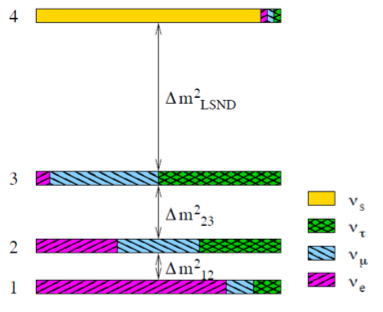
\includegraphics[width=0.95\textwidth]{./images/beyond3nu/etc/3p1.png}
  \end{column}
  \begin{column}{0.50\textwidth}
    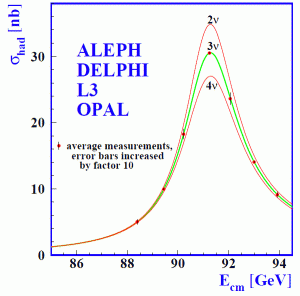
\includegraphics[width=0.95\textwidth]{./images/beyond3nu/etc/zwidth.png}
  \end{column}
\end{columns}
\begin{center}
 {\bf \color{red} A 4$^{th}$ light neutrino would have to be sterile}
\end{center}
\end{frame}

%
%
%

\begin{frame}{PMNS matrix unitarity}

    \begin{center}
      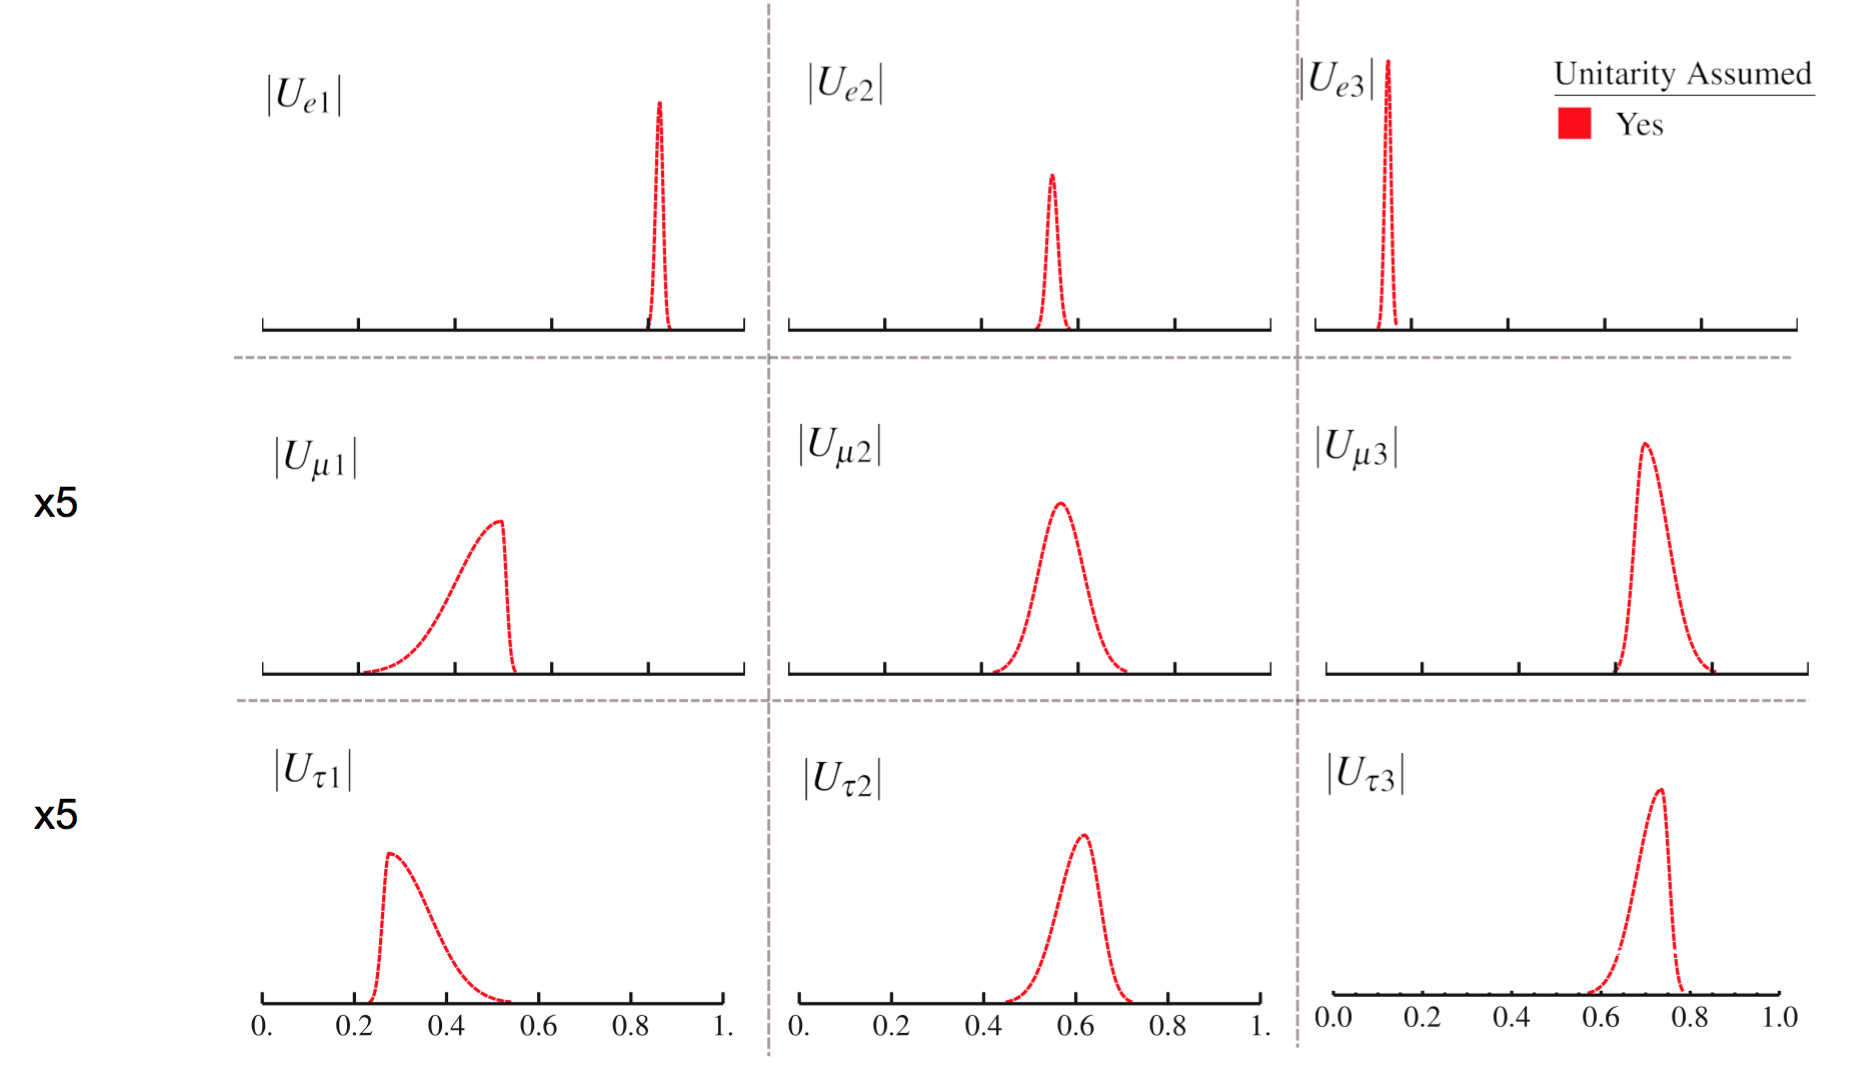
\includegraphics[width=0.88\textwidth]{./images/osc101/upmns_unitarity}\\
    \end{center}

\end{frame}

%
%
%

\begin{frame}{PMNS matrix unitarity}

    \begin{center}
      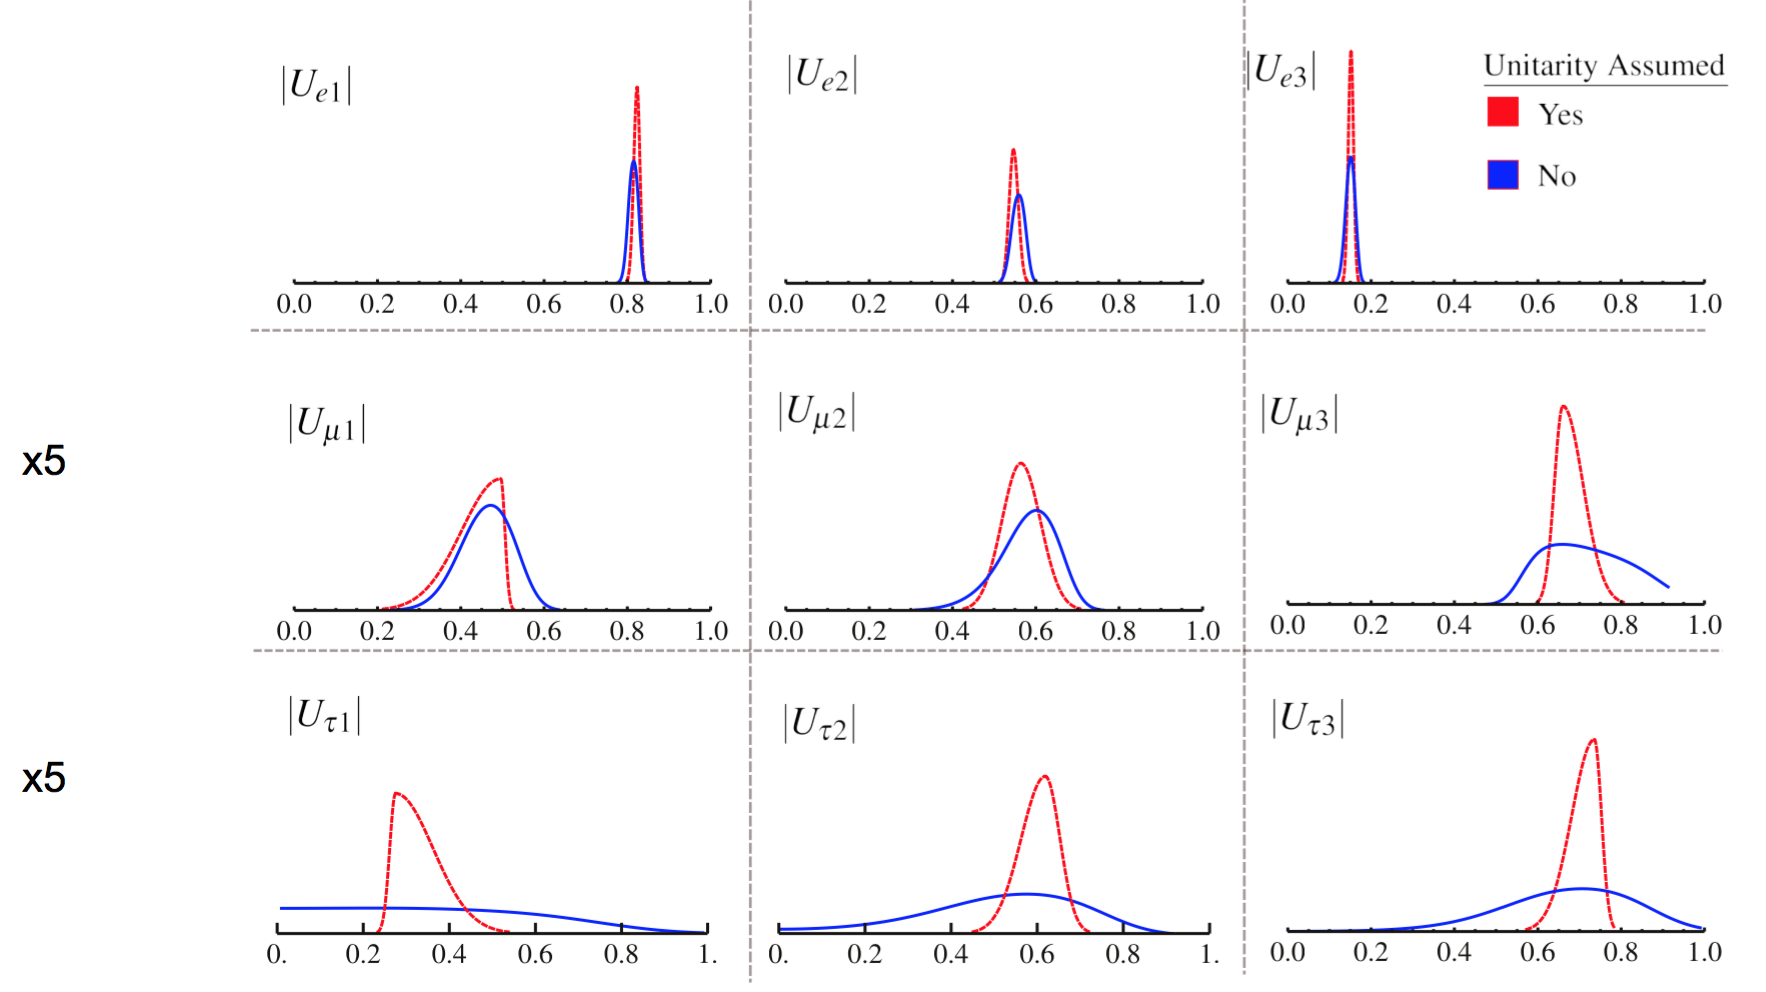
\includegraphics[width=0.88\textwidth]{./images/osc101/upmns_no_unitarity}\\
    \end{center}

\end{frame}

%
%
%

\begin{frame}{PMNS matrix unitarity}

    \begin{center}
      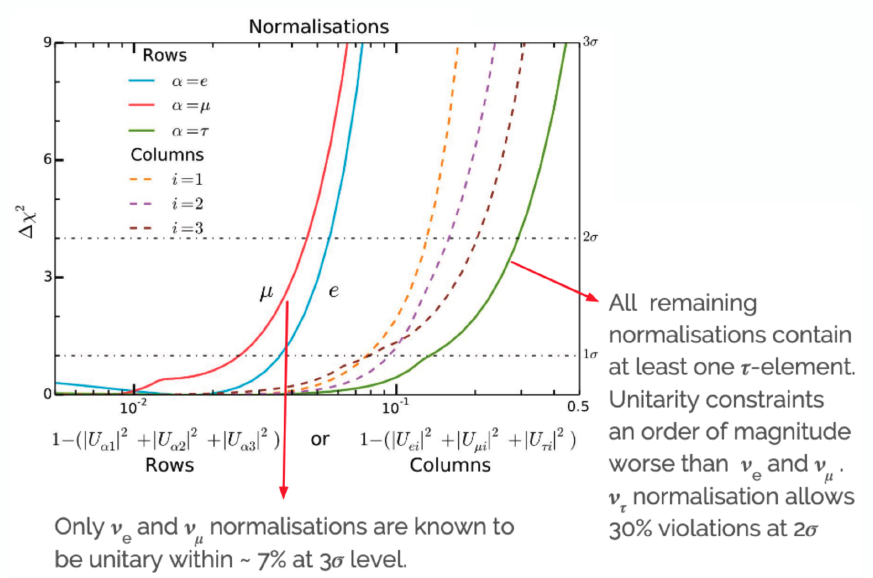
\includegraphics[width=0.88\textwidth]{./images/osc101/unitarity_limits}\\
    \end{center}
    \vspace{0.2cm}
    {\scriptsize \color{blue}[Mark Ross-Lonergan, NuFact 2016]}
\end{frame}
%
%
%

\begin{frame}[t]{Sterile neutrino phenomenology}

Mixing between active and sterile neutrinos?

\begin{center}
  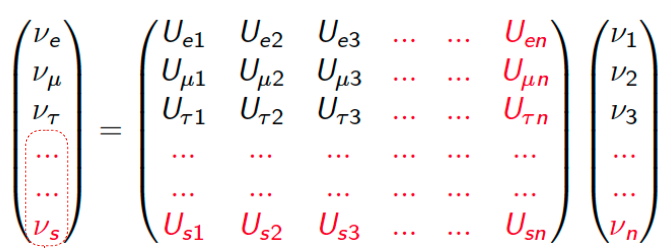
\includegraphics[width=0.88\textwidth]{./images/osc101/bigger_pmns}\\
\end{center}

The existence of such gauge singlets is well motivated and is a
natural consequence of a non-zero neutrino mass.\\

\vspace{0.2cm}

There is no a priori scale for the mass of these gauge singlets.

\end{frame}

%
%
%

\begin{frame}[t]{Sterile neutrino phenomenology}

  \begin{center}
    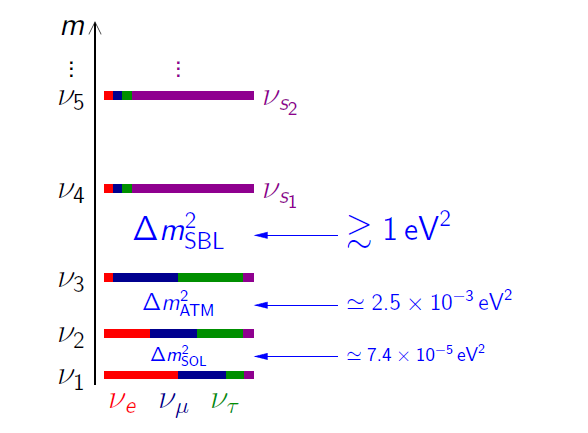
\includegraphics[width=0.88\textwidth]{./images/osc101/3p2_mass_states}\\
  \end{center}

\end{frame}

%
%
%

\begin{frame}[t]{3+1 sterile neutrino phenomenology}

\begin{itemize}
{\small
\item {\bf \color{red} $\pbar{\nu}_{e}$ disappearance}
     \[
        \displaystyle
        P(\pbar{\nu}_{e} \nrightarrow \pbar{\nu}_{e})     = 1 - sin^{2}(2\theta_{ee})    {\cdot}sin^{2}(\frac{{\Delta}m^{2}_{41}}{4E_{\nu}}),\hspace{0.1cm}
        {\color{red}sin^{2}(2\theta_{ee})} = 4 {\color{red}|U_{e4}|^{2}} \cdot (1-{\color{red} |U_{e4}|^{2}})
     \]
\item {\bf \color{blue} $\pbar{\nu}_{\mu}$ disappearance}
     \[
        \displaystyle
        P(\pbar{\nu}_{\mu} \nrightarrow \pbar{\nu}_{\mu}) = 1 - sin^{2}(2\theta_{\mu\mu}){\cdot}sin^{2}(\frac{{\Delta}m^{2}_{41}}{4E_{\nu}}),\hspace{0.1cm}
        {\color{blue}sin^{2}(2\theta_{\mu\mu})} = 4 {\color{blue}|U_{{\mu}4}|^{2}} \cdot (1-{\color{blue}|U_{{\mu}4}|^{2}})
     \]
\item {\bf \color{green} $\pbar{\nu}_{e}$ appearance in $\pbar{\nu}_{\mu}$ beam}
     \[
        \displaystyle
        P(\pbar{\nu}_{\mu} \nrightarrow \pbar{\nu}_{e})   = 1 - sin^{2}(2\theta_{{\mu}e}){\cdot}sin^{2}(\frac{{\Delta}m^{2}_{41}}{4E_{\nu}}),\hspace{0.1cm}
        {\color{green}sin^{2}(2\theta_{{\mu}e})} = 4 {\color{red} |U_{e4}|^{2}} \cdot {\color{blue} |U_{{\mu}4}|^{2}}
     \]
}
\end{itemize}
\begin{center}
Relation between appearance and disappearance channels:\\
\underline{$\pbar{\nu}_{\mu} \rightarrow \pbar{\nu}_{e}$ appearance requires $\pbar{\nu}_{\mu}$ and $\pbar{\nu}_{e}$ disappearance.}
\end{center}
\end{frame}

%
%
%

\begin{frame}[t]{The LSND experiment}

{\scriptsize
Liquid Scintillator Neutrino Detector (LSND) experiment (Los Alamos, 1993-1998) using a neutrino beam
from $\pi^{+}$ decay at rest {\color{blue}[Athanassopoulos et al., NIM A388 (1997) 149-172]}.\\
}
\begin{columns}
  \begin{column}{0.50\textwidth}
   \begin{center}
    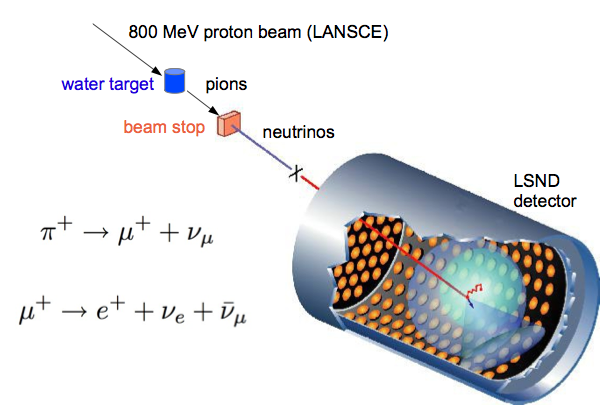
\includegraphics[width=0.90\textwidth]{./images/beyond3nu/accelerator/lsnd.png}\\
    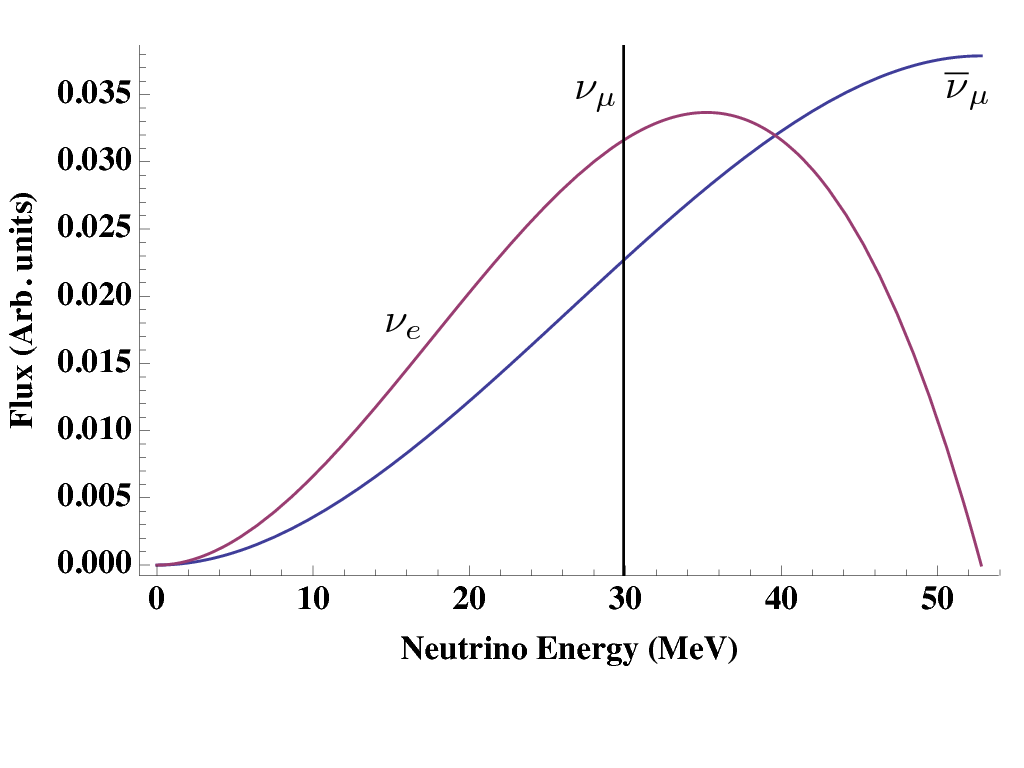
\includegraphics[width=0.70\textwidth]{./images/beyond3nu/accelerator/dar_flux.png}\\
   \end{center}
  \end{column}
  \begin{column}{0.50\textwidth}
    \begin{itemize}
    {\scriptsize
     \item 0.8-MW 800-MeV p beam % (at 120 Hz, 600 $\mu$s-long pulses)
     \item Copious amounts of pions produced in interactions with a water target
     \item $\pi^{+}$ come to rest and decay
     \item Only a small fraction of $\pi^{+}$ (3.4\%) decayed in flight
     \item $\pi^{-}$/$\pi^{+}$ $\sim$ 1/8 and most $\pi^{-}$ (and $\mu^{-}$) are absorbed before decaying.
     \item Flux shape determined simply from $\pi$, and $\mu$ decay and is well known.
     \item Homogenous mineral oil (167 tonnes) detector viewed by 1220 photomultiplier tubes (isotropic scintillation light + directional Cherenkov light cone)
     \item At a baseline of $\sim$30m (L/E $\sim$ 1m/MeV)
     \item $\bar{\nu}_{e}$ detection: Prompt $e^{+}$ signal ({\color{red}$\bar{\nu}_{e}$ + p $\rightarrow$ $e^{+}$ + n})
           followed by a correlated signal from n capture ({\color{red}n + p $\rightarrow$ d + $\gamma$} (2.2 eV))\\
%    \item No $e^{-},e^{+}$ separation, but $e^{-}$ from $\nu_{e}+^{12}C$ with energies $<$36 MeV.
    }
    \end{itemize}
  \end{column}
\end{columns}

\end{frame}

\begin{frame}[t]{The LSND anomaly}

\begin{center}
{\bf $\sim$3.8$\sigma$ $\bar{\nu}_{e}$ appearance in a beam of $\bar{\nu}_{\mu}$ from $\mu$ decay at rest\\
($\nu_{\mu}$ energy $<$ 52.8 eV) at a baseline of $\sim$30 m (L/E $\sim$ 0.7 m/MeV)}\\
\end{center}
\begin{columns}
  \begin{column}{0.50\textwidth}
    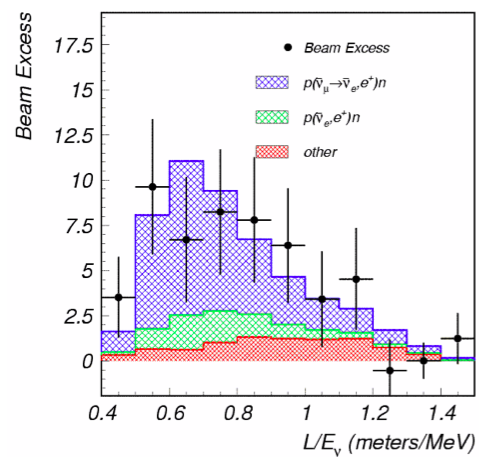
\includegraphics[width=0.90\textwidth]{./images/beyond3nu/accelerator/lsnd_excess.png}\\
  \end{column}
  \begin{column}{0.50\textwidth}
  {\small
    Main backgrounds:\\
    \begin{itemize}
    {\small
     \item ${\mu}^{-}$ decay at rest\\
%           ($\bar{\nu}_{e}$ from $\pi^{-} \rightarrow \mu^{-}+\bar{\nu}_{\mu};
%            \mu^{-} \rightarrow e^{-}+\bar{\nu}_{e}+\nu_{\mu}$)
           followed by $\bar{\nu}_{e}$ + p $\rightarrow$ $e^{+}$ + n
     \item ${\pi}^{-}$ decay in flight\\
           followed by $\bar{\nu}_{\mu}+p \rightarrow \mu^{+}+n$\\
    }
    \end{itemize}
    \vspace{0.1cm}
    {\centering
      {\bf $\bar{\nu}_{e}$ excess observed:}\\
         {\bf \color{red}87.9 $\pm$ 22.4 (stat) $\pm$ 6 (syst)}\\
      \vspace{0.1cm}
      Under a 2-$\nu$ mixing hypothesis:\\
      {\color{red}$P(\bar{\nu_{\mu}} \rightarrow \bar{\nu_{e}})$ = 0.264  $\pm$ 0.067  $\pm$ 0.045 \%} \\
    }
  }
  \end{column}
\end{columns}
\begin{center}
 {\scriptsize \color{blue}[Aguilar-Arevalo, RD64 (2001) 112007]}\\
\end{center}
\end{frame}


%
%
%

\begin{frame}[t]{But no significant $\bar{\nu}_{e}$ excess seen in KARMEN}

\begin{columns}
  \begin{column}{0.35\textwidth}
  {\scriptsize
    At the same time with LSND, a very similar experiment (KARMEN) using a segmented liquid scintillation calorimeter
    was run at the Rutherford Appleton Laboratory exploiting the distinct time structure of the ISIS source
    {\color{blue}[Drexlin et al., NIM A289 (1990) 490-495]}. \\
    \vspace{0.5cm}
    KARMEN found no evidence for a $\bar{\nu}_{e}$ excess
    {\color{blue}[Armbruster et al., Phys.Rev. D65 (2002) 112001]}.\\
    \vspace{0.5cm}
    However the KARMEN and LSND results were not incompatible (under a 2-neutrino oscillation hypothesis).\\
  }
  \end{column}
  \begin{column}{0.65\textwidth}
    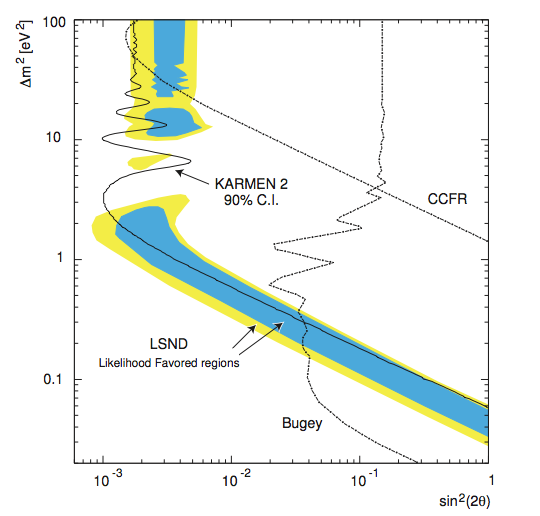
\includegraphics[width=0.95\textwidth]{./images/beyond3nu/accelerator/lsnd_karmen_combined.png}
  \end{column}
\end{columns}
\end{frame}


%
%
%

\begin{frame}[t]{Testing the LSND oscillation hypothesis: MiniBooNE}

{\small
MiniBooNE experiment:
\begin{itemize}
 {\small
  \item Keeping the same L/E ratio, but perform an indpendent experiment at a different energy range,
        with different event signature / backgrounds and different systematics\\
  \item Detector: 800 tonnes of mineral oil instrumented with 1280 photosensors\\
  \item $\sim$500 m from the target, at the Booster neutrino beam at Fermilab\\
 }
\end{itemize}
}
\begin{center}
 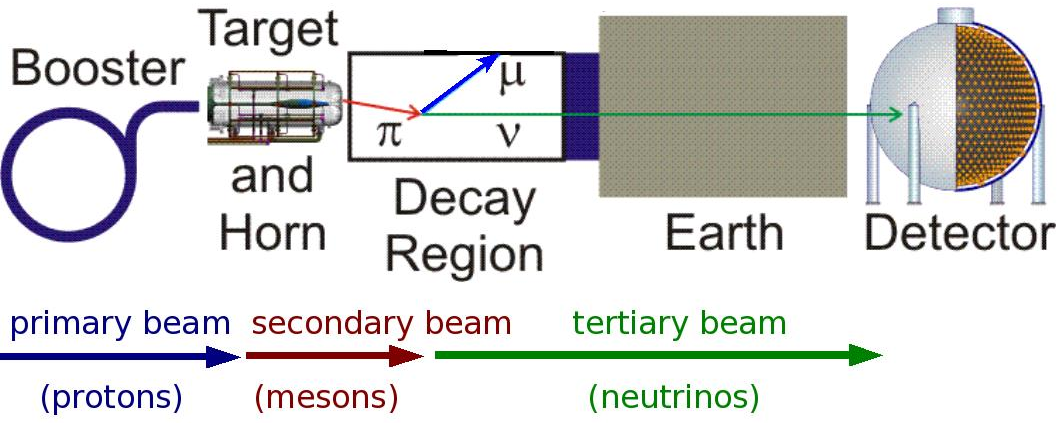
\includegraphics[width=0.80\textwidth]{./images/beyond3nu/accelerator/miniboone.png}\\
\end{center}
\end{frame}

%
%
%

\begin{frame}[t]{MiniBooNE results}

\begin{columns}[T]
  \begin{column}{0.55\textwidth}
    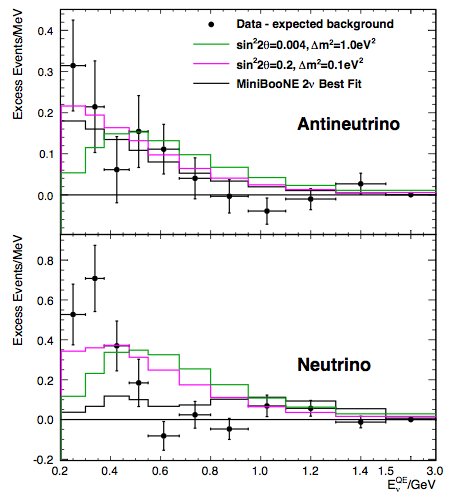
\includegraphics[width=0.90\textwidth]{./images/beyond3nu/accelerator/miniboone_osc_results_spectra.png}
    \vspace{0.1cm}
    {\scriptsize \color{blue}[Phys. Rev. Lett. 110, 161801 (2013)]}\\
  \end{column}
  \begin{column}{0.35\textwidth}
    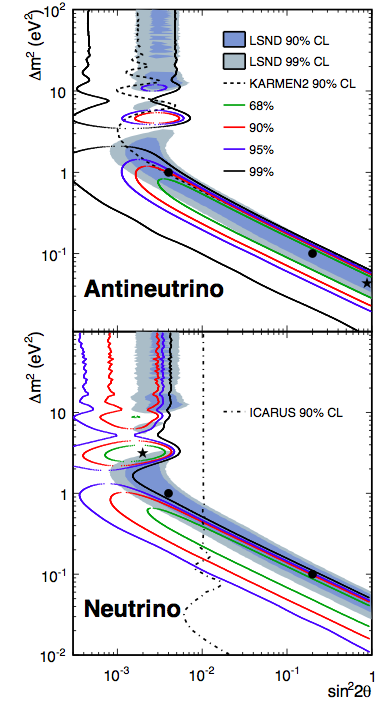
\includegraphics[width=0.99\textwidth]{./images/beyond3nu/accelerator/miniboone_osc_results_contours.png}
  \end{column}
\end{columns}
\end{frame}

%
%
%

\begin{frame}[t]{Updated MiniBooNE results (2018)}

  \begin{columns}[T]
    \begin{column}{0.55\textwidth}
      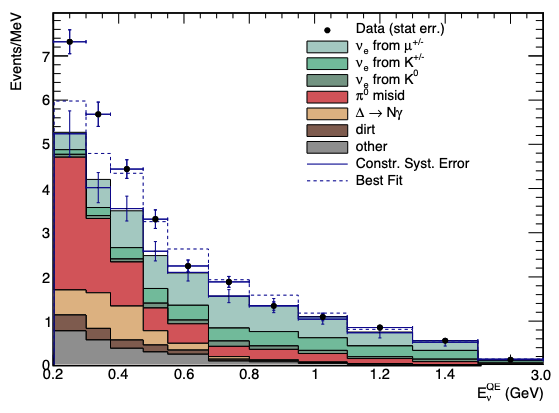
\includegraphics[width=0.95\textwidth]{./images/beyond3nu/accelerator/miniboone_new_excess}
    \end{column}
    \begin{column}{0.45\textwidth}
      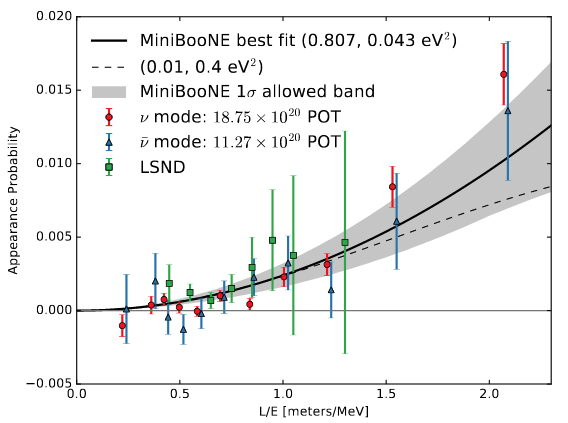
\includegraphics[width=0.99\textwidth]{./images/beyond3nu/accelerator/miniboone_new_app_prob}
      \vspace{-0.2cm}
      \begin{center}
      {\scriptsize \color{blue}[Phys.Rev.Lett. 121 (2018) 22, 221801]}\\
      {\scriptsize \color{blue}[Phys.Rev.D 103 (2021) 5, 052002]}\\
      \end{center}
    \end{column}
  \end{columns}

  \begin{itemize}
    \item Additional data (1.127$\times$10$^{21}$ pot, 46\% increase)
    \item Total excess of 638.0 $\pm$ 52.1(stat.) $\pm$ 122.2(syst.)
    \item Overall significance 4.8$\sigma$
  \end{itemize}
\end{frame}


%
%
%

\begin{frame}[t]{New MicroBooNE single photon results (2021)}

{\small
Disfavours $\Delta \rightarrow N \gamma$ as the explanation of the MiniBooNE anomaly at 94.8\% CL.\\
{\scriptsize \color{blue}[arXiv:2110.00409]}\\
}
\vspace{-0.3cm}
\begin{columns}[T]
    \begin{column}{0.50\textwidth}
    \begin{center}
      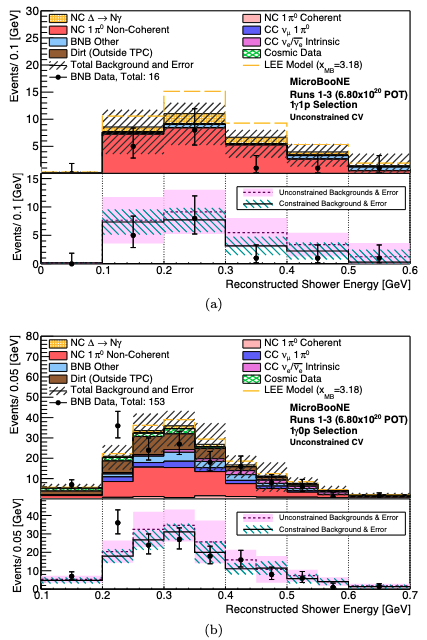
\includegraphics[width=0.70\textwidth]{./images/beyond3nu/accelerator/uB_2021_gamma_0}
    \end{center}
    \end{column}
    \begin{column}{0.50\textwidth}
    \begin{center}
      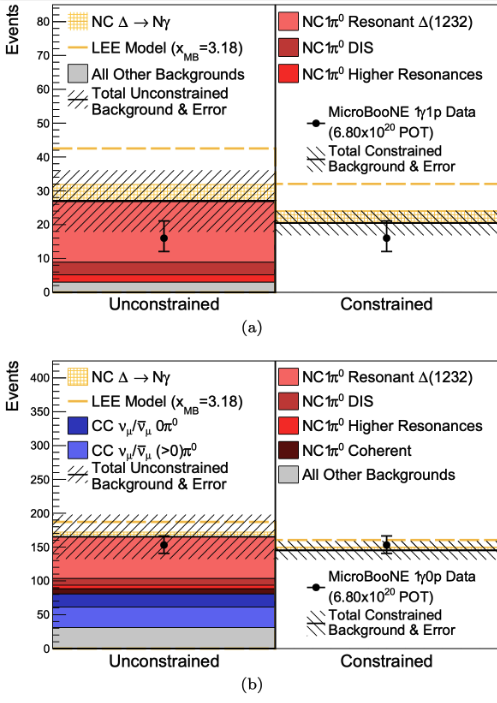
\includegraphics[width=0.80\textwidth]{./images/beyond3nu/accelerator/uB_2021_gamma_1}
    \end{center}
    \end{column}
\end{columns}

\end{frame}

%
%
%

\begin{frame}[t]{New MicroBooNE single electron results (2021)}

  \begin{center}
    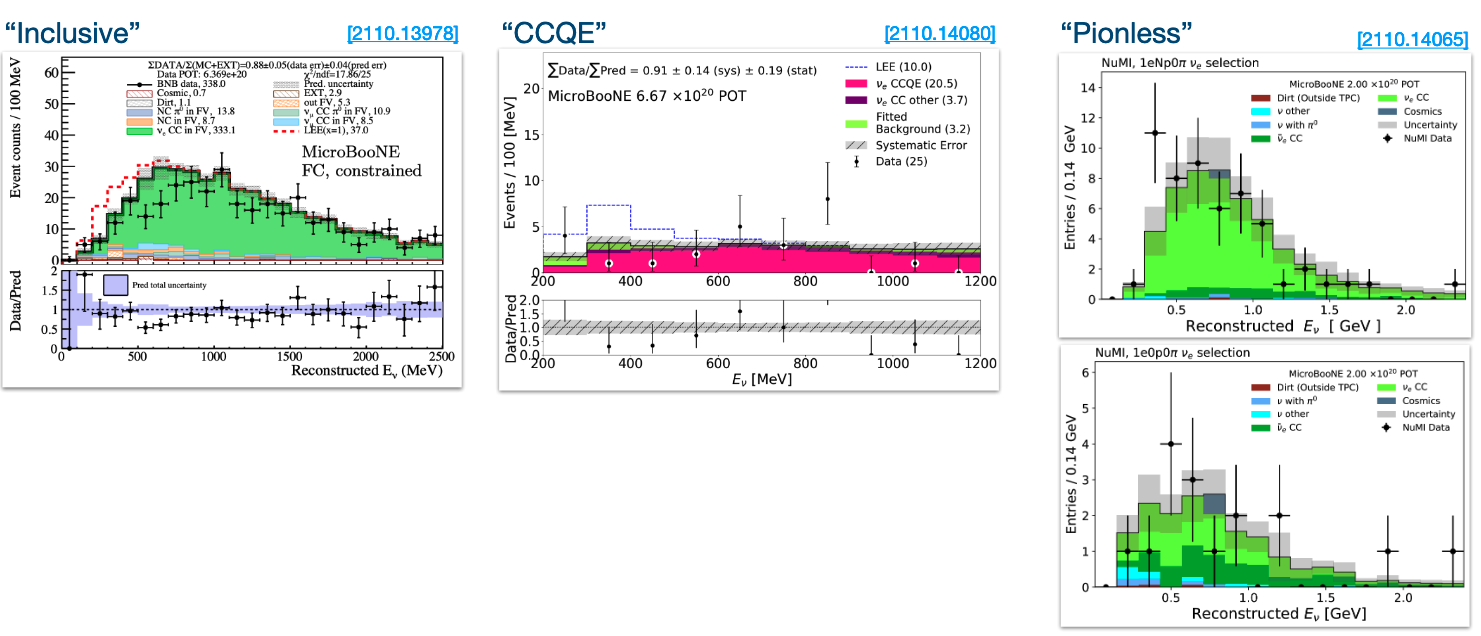
\includegraphics[width=0.99\textwidth]{./images/beyond3nu/accelerator/uB_2021_e_x3}
  \end{center}

\end{frame}

\begin{frame}[t]{New MicroBooNE single electron results (2021)}

{\small
  "Results are found to be consistent with the nominal electron neutrino
  rate expectations from the Booster Neutrino Beam and no excess of electron neutrino events is observed".\\
}
\vspace{0.1cm}

\begin{center}
    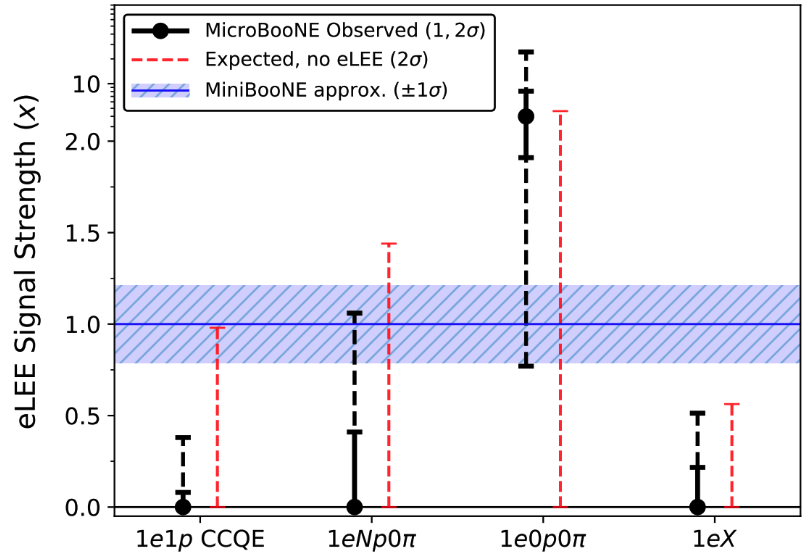
\includegraphics[width=0.70\textwidth]{./images/beyond3nu/accelerator/uB_2021_e_summary}
\end{center}

\end{frame}
%
%
%

\begin{frame}[t]{Multi-GeV $\nu_{e}$ and $\bar{\nu}_{e}$ appearance searches}

\begin{columns}
  \begin{column}{0.40\textwidth}
    \begin{itemize}
      \item Recent results from the ICARUS and OPERA experiments at the CERN CNGS beam.
      \item No evidence for $\nu_{e}$ appearance in multi-GeV $\nu_{\mu}$ beam.
      \item Cutting away at the LSND+MiniBooNE region.
      \item Global fit to appearance data still consistent with oscillations.
    \end{itemize}
  \end{column}
  \begin{column}{0.60\textwidth}
    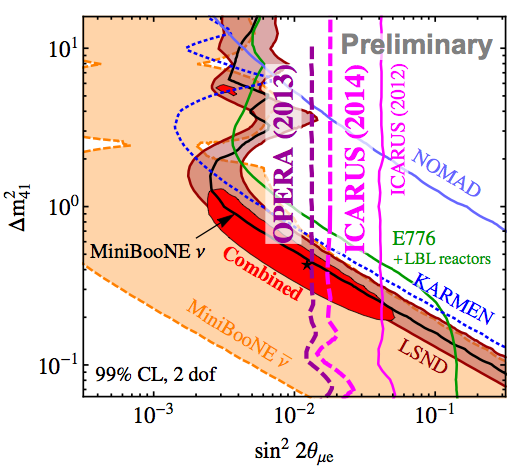
\includegraphics[width=0.95\textwidth]{./images/beyond3nu/pheno/kopp_global_app_withcngs.png}\\
    {\color{blue}[Kopp, Neutrino 2014 conference, Boston]}.
  \end{column}
\end{columns}
\end{frame}

%
%
%

\begin{frame}[t]{Recent $\nu_{\mu}$ and $\bar{\nu}_{\mu}$ disappearance searches}

\begin{columns}
  \begin{column}{0.50\textwidth}
   \centering
    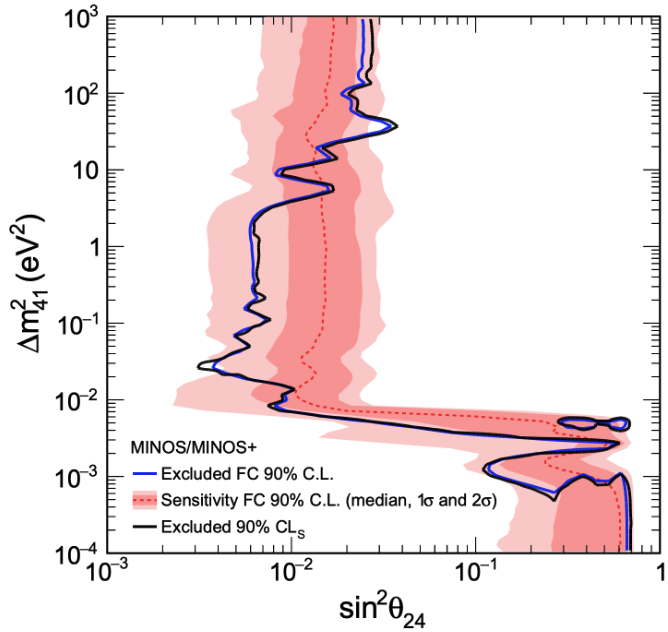
\includegraphics[width=0.99\textwidth]{./images/beyond3nu/minos_sterile_disapp_recent}\\
    {\color{blue}[arXiv:2002.00301]}.
  \end{column}
  \begin{column}{0.50\textwidth}
    \centering
     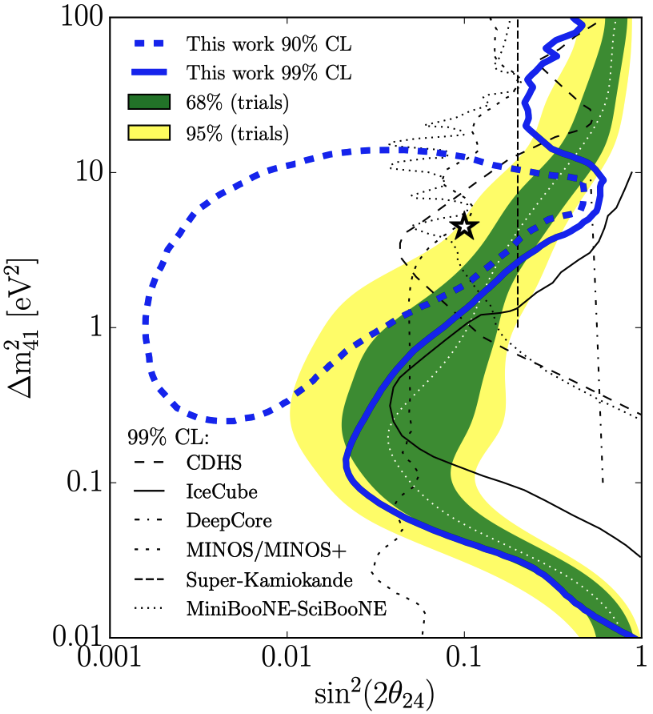
\includegraphics[width=0.90\textwidth]{./images/beyond3nu/icecube_sterile_disapp_recent}\\
     {\color{blue}[arXiv:2005.12942]}.
  \end{column}
\end{columns}
\end{frame}

%
%
%

\begin{frame}[t]{The reactor anomaly}

Recent re-evaluation of the predicted reactor neutrino flux (+3.5\%), accounting of long-lived isotopes (+1\%)
and new measurements of  the neutron lifetime impacting the inverse beta decay cross-section (+1.5\%).\\
\vspace{0.3cm}
Experimental results now sitting about 3$\sigma$ lower than predictions.\\
\vspace{0.2cm}
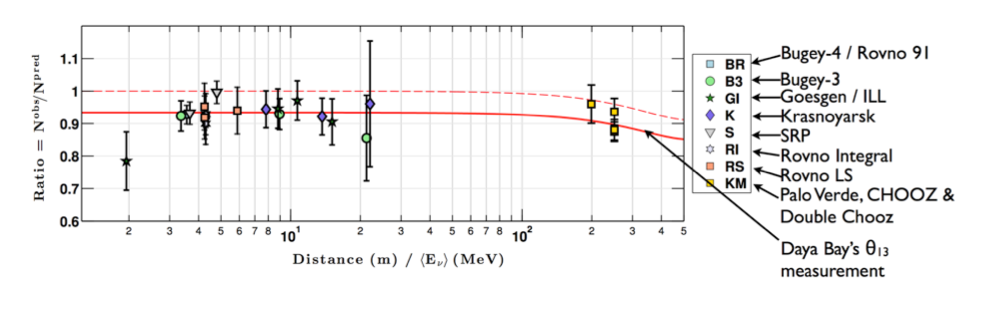
\includegraphics[width=0.95\textwidth]{./images/beyond3nu/reactor/deficit2.png}\\
{\scriptsize \color{blue}
 Mention et al., Phys. Rev. D 83 073006 (2011);
 Mueller et al., Phys. Rev. C 83, 054615 (2011);
 P. Huber, Phys. Rev. C 84, 024617 (2011);
 Hayes et al, Phys. Rev Le1. 112,202501 (2014)
}

\end{frame}

%
%
%

\begin{frame}[t]{The Gallium anomaly}

\begin{columns}
  \begin{column}{0.60\textwidth}
  \begin{itemize}
   \item Tests of (the detection efficiency of the) GALLEX and SAGE radiochemical solar neutrino detectors
   \item Neutrino detection via $\nu_{e}$ + $^{71}$Ga $\rightarrow$ $e^{-}$ + $^{71}$Ge
   \item 4 runs using intense (0.6 - 2 MCi) radioactive (electron capture) $\nu_{e}$ sources
         ($^{51}$Cr (750 keV) and $^{37}$Ar (810 keV))
   \item GALLEX: $^{51}$Cr, $<L>$=1.9m.
   \item SAGE: $^{51}$Cr and $^{37}$Ar, $<L>$=0.6m.
  \end{itemize}
  \end{column}
  \begin{column}{0.40\textwidth}
    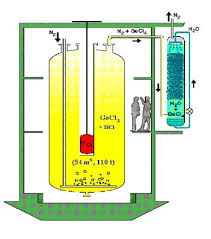
\includegraphics[width=0.95\textwidth]{./images/beyond3nu/gallium/gallex.jpg}
  \end{column}
\end{columns}
\end{frame}

%
%
%

\begin{frame}[t]{The Gallium anomaly}

A deficit was observed:\\
\begin{table}[ht]
 \centering
 \begin{tabular}{| c | c | c | c |}
   \hline
   Experiment &  Run &  Source     & Ratio (measured/predicted) \\
   \hline
   GALLEX     &    1 &  $^{51}$Cr  & 0.953$\pm$0.11             \\
   GALLEX     &    2 &  $^{51}$Cr  & 0.812$^{+0.10}_{-0.11}$    \\
   SAGE       &    1 &  $^{51}$Cr  & 0.95$\pm$0.12              \\
   SAGE       &    2 &  $^{37}$Ar  & 0.791$^{+0.084}_{-0.078}$  \\
   \hline
 \end{tabular}
\end{table}
Combined ratio R = 0.86 $\pm$ 0.05 {\scriptsize \color{blue}[Giunti and Laveder, Phys.Rev. C83 (2011) 065504]}\\
\vspace{0.1cm}
\begin{itemize}
{\scriptsize
  \item The deficit depends on the cross-section value for the
            {\color{red}$\nu_{e}$ + $^{71}$Ga $\rightarrow$ $e^{-}$ + $^{71}$Ge} process.
  \item The cross-section for the transition from the ground state of $^{71}$Ga to the ground state of
            $^{71}$Ge is known precisely from the electron capture decay rate of $^{71}$Ge.
  \item  However, $\nu_{e}$ from the sources used at GALLEX and SAGE may be absorbed by $^{71}$Ga
             with transitions to excited states of $^{71}$Ge (175 keV,
             500 keV)
             \begin{itemize}
                 {\scriptsize
                    \item Inferred from: p + $^{71}$Ga $\rightarrow$ n + $^{71}$Ge.
                    \item Supported by recent data {\color{blue}[Frekers et al.,Phys.Lett. B706 (2011) 134-138]}
                 }
             \end{itemize}
}
\end{itemize}
\end{frame}


%\begin{frame}[t]{Tensions between datasets}
%
%\begin{center}
%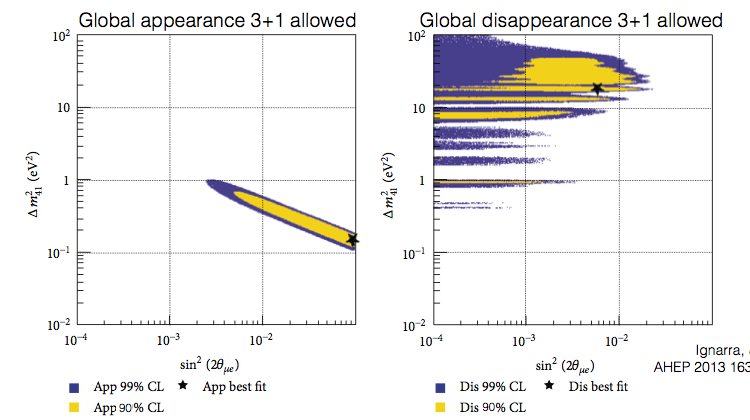
\includegraphics[width=0.95\textwidth]{./images/beyond3nu/pheno/tension_app_disapp.png}
%\end{center}
%\end{frame}


%\begin{frame}[t]{Tensions between datasets}
%
%\begin{center}
%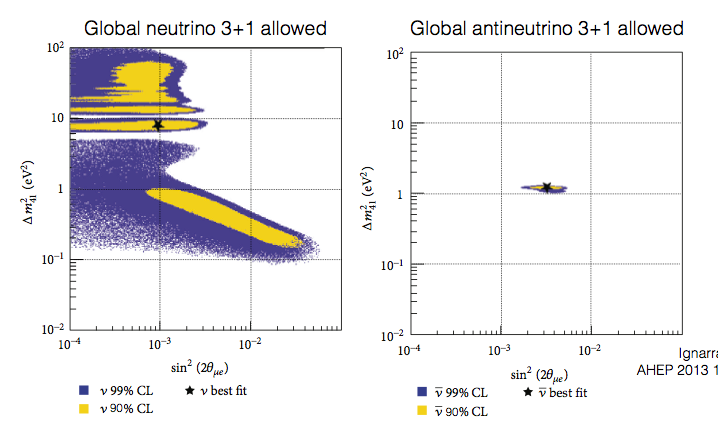
\includegraphics[width=0.95\textwidth]{./images/beyond3nu/pheno/tension_nu_nubar.png}
%\end{center}
%\end{frame}


%\begin{frame}[t]{Sterile neutrino phenomenology}
%
%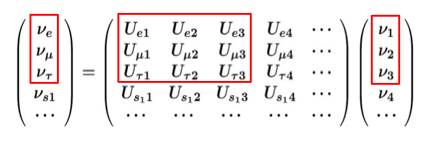
\includegraphics[width=0.45\textwidth]{./images/beyond3nu/pheno/sterile_pmns_2.png}\\
%\end{frame}



\begin{frame}[t]{Global sterile neutrino fits}

\begin{columns}
  \begin{column}{0.70\textwidth}
    \centering
     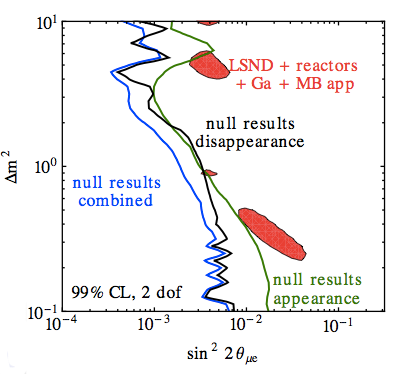
\includegraphics[width=0.90\textwidth]{./images/beyond3nu/pheno/global3p1.png}\\
     {\scriptsize \color{blue}[Kopp, Machado, Maltoni and Schwetz, JHEP 1305 (2013) 050]}
  \end{column}
  \begin{column}{0.30\textwidth}
    {\small
     \centering
      We saw {\color{blue}$\nu_{e}$ disappearance} and {\color{blue}$\nu_{\mu} \rightarrow \nu_{e}$ appearance}
      but no {\color{red}$\nu_{\mu}$ disappearance}\\
      \vspace{0.2cm}
      {\bf Severe tension between datasets} in a 3+1 framework\\
      \vspace{0.2cm}
      Tension relieved somewhat with more complex models, but...\\
      \vspace{0.2cm}
      However the implications are just too important to ignore.\\
    }
  \end{column}
\end{columns}
\end{frame}


\begin{frame}[plain,c]
\begin{center}
{\Large To address the question of the \\
potential existence of eV-scale sterile neutrino (or other BSM physics)\\
we need data from experiments\\ with {\bf compelling [*]} sensitivity}\\
\vspace{2cm}
[*] The definition of {\em compelling} is subjective. In my view, {\bf $\sim$10$\sigma$ exclusion} of the allowed range is needed
by proposals likely to produce the data to settle the issue. Such proposals exist.
\end{center}
\end{frame}

\begin{frame}[plain,c]
\begin{center}
  Several new theoretical ideas are put forward\\
  \vspace{0.2cm}
  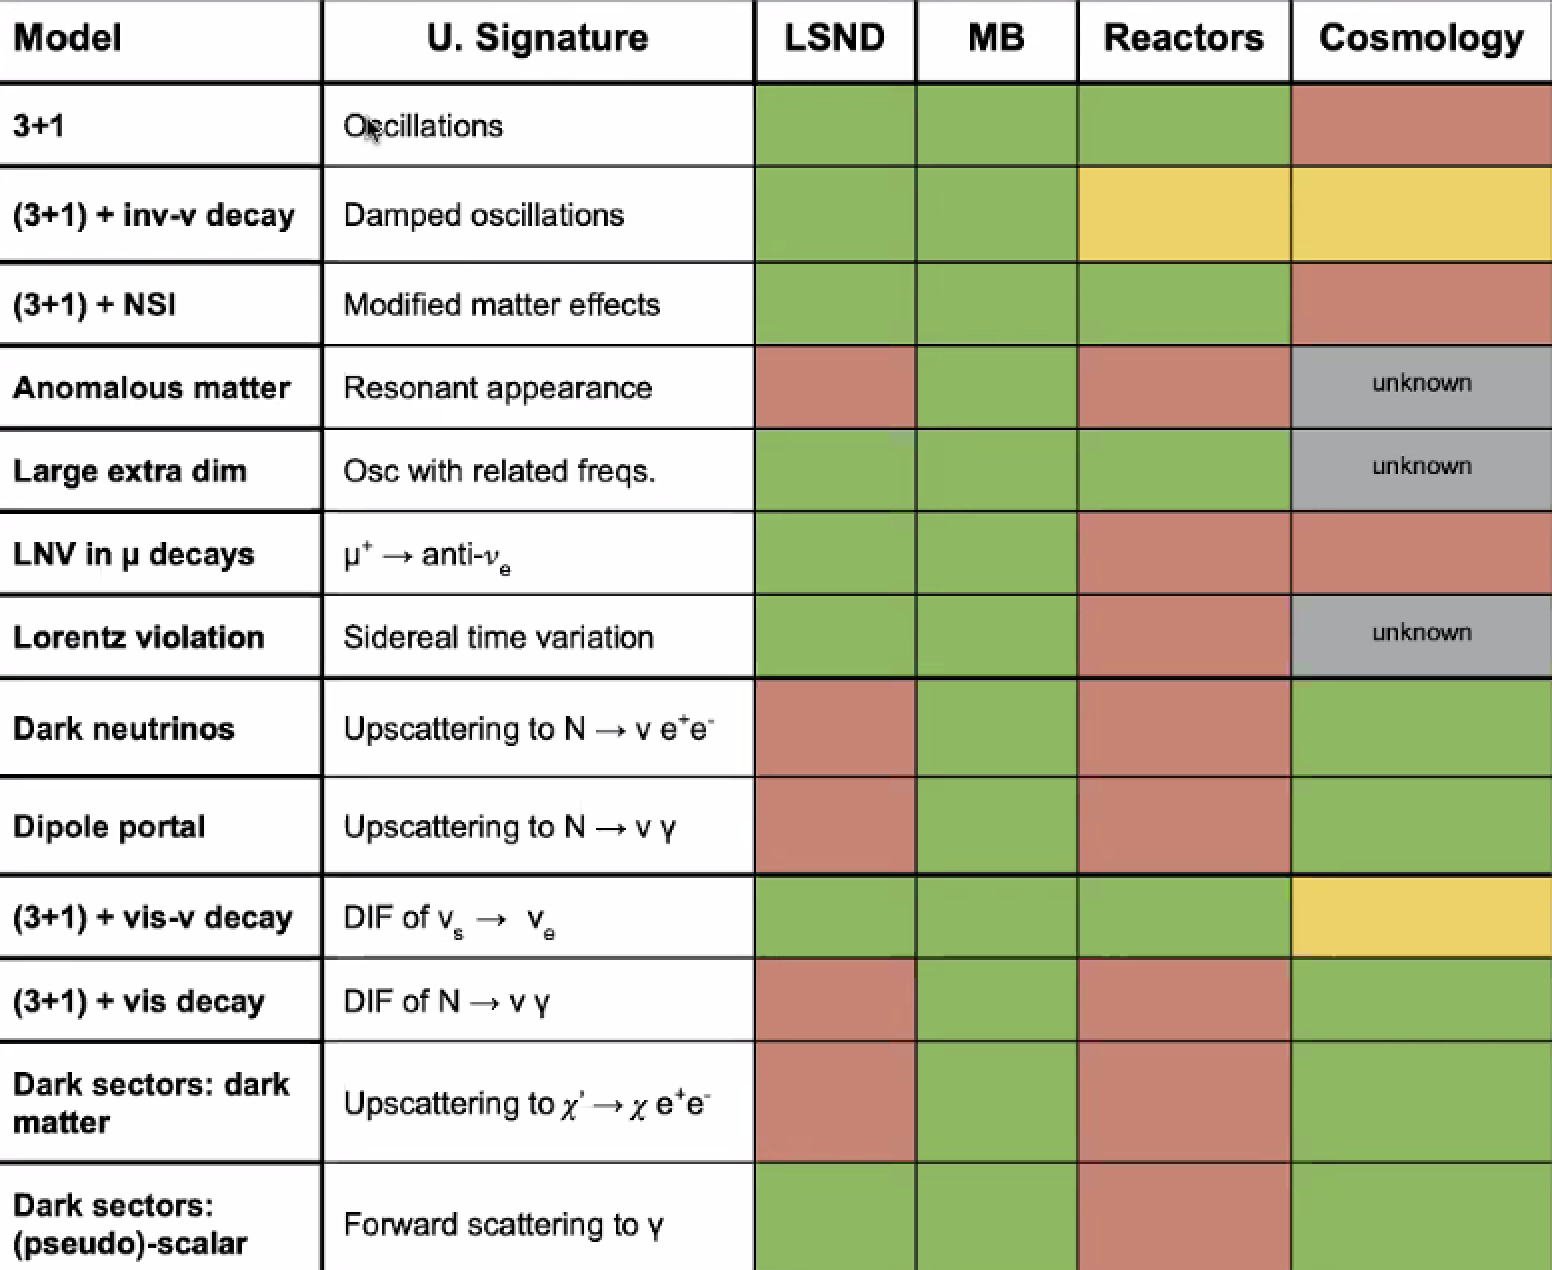
\includegraphics[width=0.90\textwidth]{./images/beyond3nu/new_models}
\end{center}
\end{frame}


\begin{frame}[t]{Future searches}

\begin{itemize}
\item Accelerator facilities
\item Source experiments
\item Reactor experiments
\end{itemize}

\end{frame}


\begin{frame}[t]{Future accelerator based projects}

\begin{itemize}
   \item {\bf $\pi$,$\mu$   decay at rest}
     \begin{itemize}
        \item OscSNS, JPARC MLF
     \end{itemize}
   \item {\bf Isotope decay at rest}
     \begin{itemize}
         \item IsoDAR@KamLAND
     \end{itemize}
   \item {\bf $\pi$,K decay in flight}
     \begin{itemize}
          \item LAr1-ND, MicroBooNE, ICARUS@FNAL
     \end{itemize}
   \item {\bf $\mu$ decay in flight}
     \begin{itemize}
           \item $\nu$Storm
     \end{itemize}
\end{itemize}

%  \begin{table}[ht]
%  \centering
%   \begin{tabular}{| c | c | c | c |}
%  \hline
% Source & Project &  Primary & Other    \\
%       &         &  channel & channels \\
%   \hline
%   $\pi$,$\mu$   decay at rest  & OscSNS          & $\bar{\nu}_{\mu} \rightarrow \bar{\nu}_{e}$ & \\
%   $\pi$,$\mu$,K decay at rest  & JPARC MLF       & & \\
%   Isotope decay at rest        & IsoDAR@KamLAND  & & \\
%   $\pi$,K decay in flight      & LAr1-ND         & & \\
%   $\pi$,K decay in flight      & MicroBooNE      & & \\
%   $\pi$,K decay in flight      & ICARUS@FNAL     & & \\
%   $\mu$ decay in flight        & $\nu$Storm      & & \\
%   \hline
%   \end{tabular}
%  \end{table}

\end{frame}



\begin{frame}[t]{Future reactor projects}
\centering
\begin{columns}
  \begin{column}{0.50\textwidth}
    \begin{itemize}
     {\scriptsize
      \item New experiments, at very short baselines, close to a single (research) reactor core
      \item Challenging environment:
               Very short baseline (reactor backgrounds) and shallow
               depths (cosmic backgrounds).\\
    }
    \end{itemize}
  \end{column}
  \begin{column}{0.50\textwidth}
     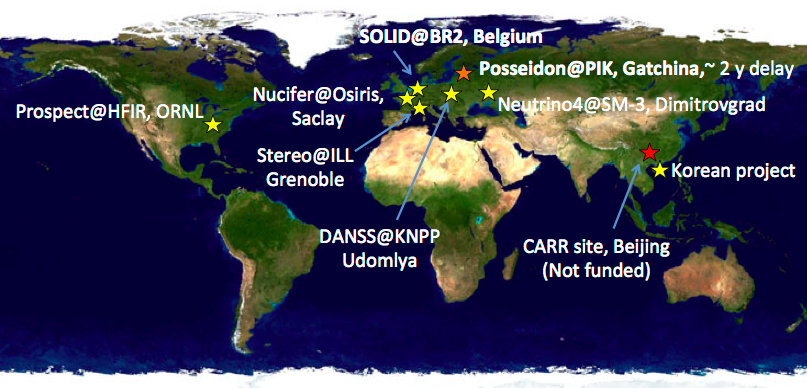
\includegraphics[width=0.90\textwidth]{./images/beyond3nu/future/vsbn_reactor_map.png}
  \end{column}
\end{columns}
\begin{columns}[t]
  \begin{column}{0.50\textwidth}
     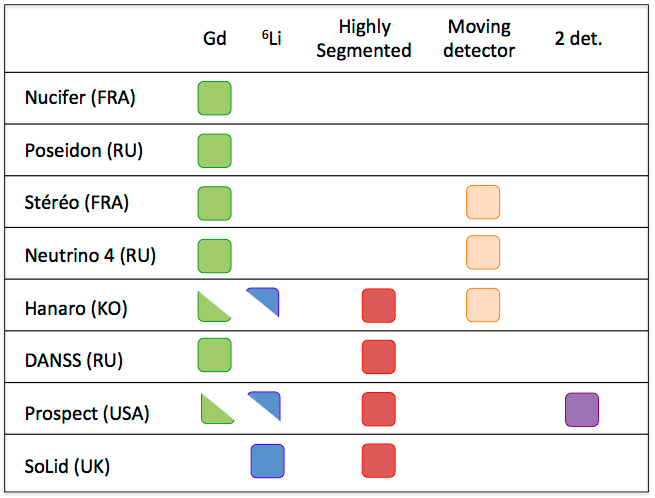
\includegraphics[width=0.90\textwidth]{./images/beyond3nu/future/vsbn_reactor_tab1.png}
  \end{column}
  \begin{column}{0.50\textwidth}
     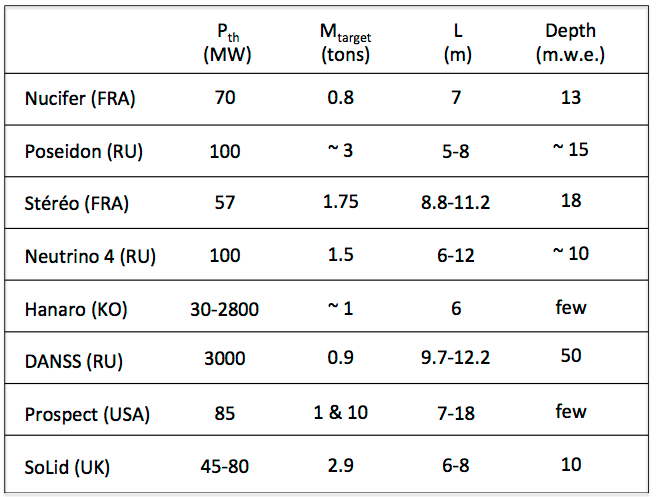
\includegraphics[width=0.95\textwidth]{./images/beyond3nu/future/vsbn_reactor_tab2.png}
  \end{column}
\end{columns}
{\scriptsize \color{blue}[schematics from David Lhuillier, Neutrino 2014 conference, Boston]}
\end{frame}


\begin{frame}[t]{Future neutrino source projects}
\centering
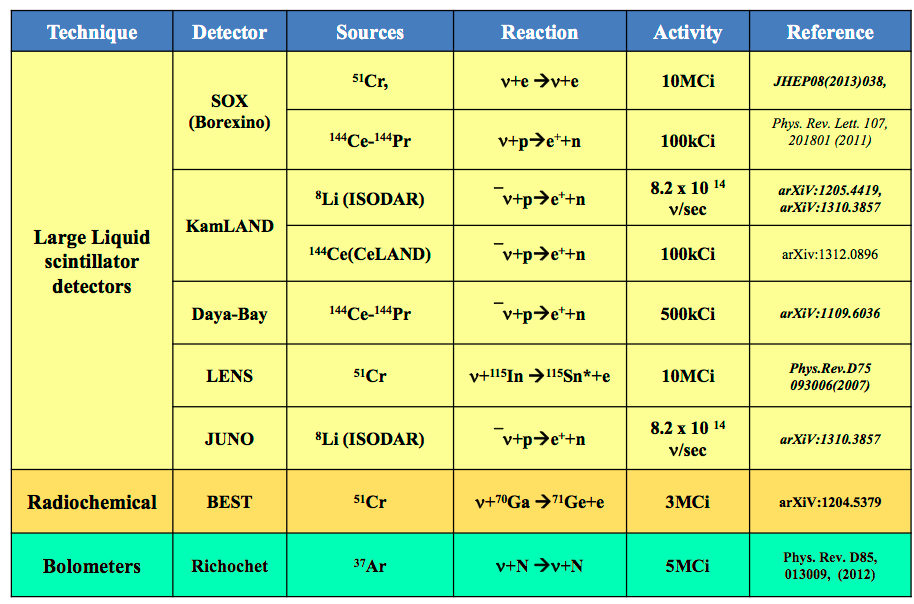
\includegraphics[width=0.88\textwidth]{./images/beyond3nu/future/hot_source_tab.png}\\
{\scriptsize \color{blue}[Barbara Caccianiga, Neutrino 2014 conference, Boston]}

\end{frame}



\begin{frame}[t]{Future accelerator-based projects: $\pi$ DAR neutrinos}

Try to solve the LSND anomaly with an improved LSND-style experiment: OscSNS
{\color{blue}[The OscSNS White Paper, arXiv:1307.7097]}
\begin{columns}
  \begin{column}{0.50\textwidth}
     \begin{itemize}
     {\scriptsize
       \item Proposed experiment using the 1.4-MW 1-GeV proton beam at
             the Oak Ridge Spallation Neutron Source.
       \item 2.2$\times$10$^{23}$ protons/yr $\rightarrow$
             2.8$\times$10$^{22}$ $\nu$/yr
       \item Short-pulses (695 ns) $\rightarrow$ reduced cosmic-ray bkg and to separate
             neutrinos from $\pi^{+}$ and $\mu^{+}$ decay.
       \item Cylindrical detector 60 m away from the beam stop,
             filled with 886 tonnes (450 tonnes fiducial)
             mineral oil and instrumented with 350 8-inch photomultiplier tubes (25\% coverage).
     }
     \end{itemize}
  \end{column}
  \begin{column}{0.50\textwidth}
    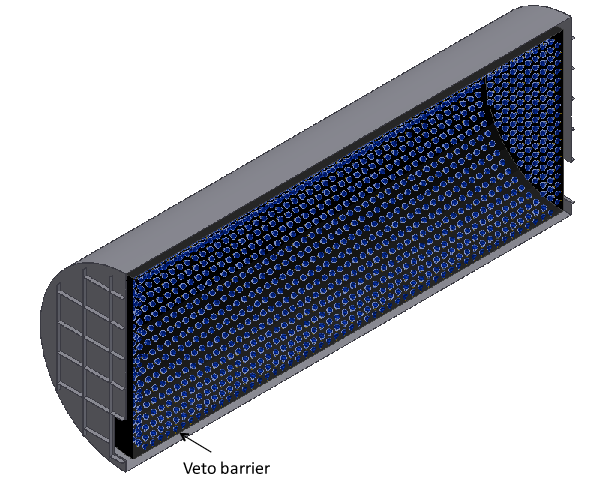
\includegraphics[width=0.95\textwidth]{./images/beyond3nu/future/oscsns_detector.png}
  \end{column}
\end{columns}
\begin{center}
{\scriptsize
 Similar experiment is being proposed at J-PARC (Japan)
 {\color{blue}[Harada et al, arXiv:1310.1437]}
}
\end{center}
\end{frame}


\begin{frame}[t]{Future accelerator-based projects: $\pi$ DAR neutrinos}

Try to solve the LSND anomaly with an improved LSND-style experiment: OscSNS
{\color{blue}[The OscSNS White Paper, arXiv:1307.7097]}
\begin{columns}
  \begin{column}{0.50\textwidth}
     \begin{itemize}
       \item {\bf $\bar{\nu}_{\mu} \rightarrow \bar{\nu}_{e}$ }\\
         {\scriptsize
           Prompt $e^{+}$ signal ({\color{red}$\bar{\nu}_{e}$ + p $\rightarrow$ $e^{+}$ + n})
           followed by a correlated signal from n capture ({\color{red}n + p $\rightarrow$ d + $\gamma$} (2.2 eV))\\
         }
       \item {\bf $\nu_{\mu} \rightarrow \nu_{e}$ }\\
         {\scriptsize
           Monoenergetic 12.5 MeV $e^{-}$
           ({\color{red}$\nu_{e}+^{12}C \rightarrow e^{-}+^{12}N$})
           followed by $e^{+}$ from the $\beta$-decay of $^{12}N$.
         }
       \item {\bf $\nu_{\mu}$ disappearance }\\
         {\scriptsize
           15.11 MeV $\gamma$ from {\color{red}$\nu_{\mu}C \rightarrow \nu_{\mu}C^{*}$}
         }
       \item {\bf $\nu_{e}$ disappearance }\\
         {\scriptsize
           {\color{red}$\nu_{e}+^{12}C \rightarrow e^{-}+^{12}N$}
           followed by $e^{+}$ from the $\beta$-decay of $^{12}N$.
         }
     \end{itemize}
  \end{column}
  \begin{column}{0.50\textwidth}
    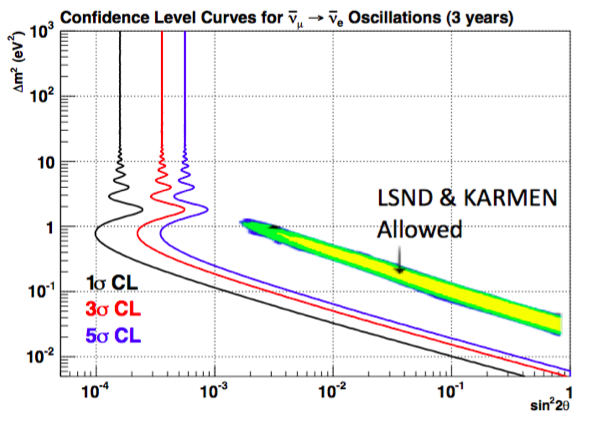
\includegraphics[width=0.95\textwidth]{./images/beyond3nu/future/oscsns_sensitivity.png}
  \end{column}
\end{columns}
\end{frame}


\begin{frame}[t]{Future accelerator-based projects: Isotope DAR neutrinos}

IsoDAR experiment:\\
Injector cyclotron setup + kton-scale scintillator-based detector

\begin{columns}
  \begin{column}{0.50\textwidth}
     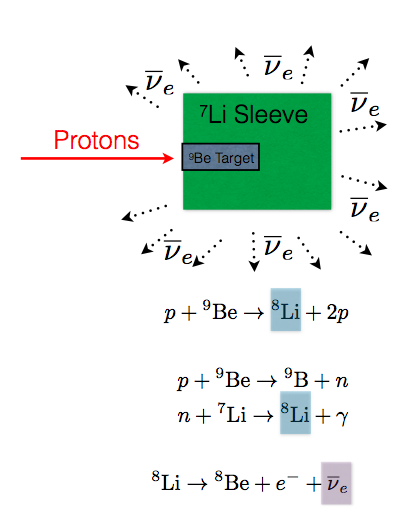
\includegraphics[width=0.75\textwidth]{./images/beyond3nu/future/isodar1.png}\\
     {\scriptsize \color{blue}[adapted from J.Spitz, Neutrino 2014, Boston]}
  \end{column}
  \begin{column}{0.50\textwidth}
     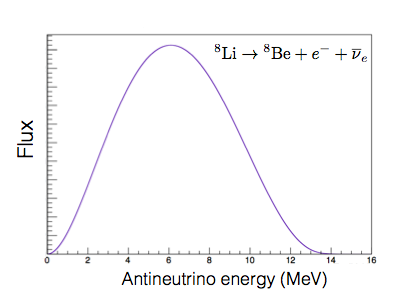
\includegraphics[width=0.80\textwidth]{./images/beyond3nu/future/isodar_flux.png}\\
     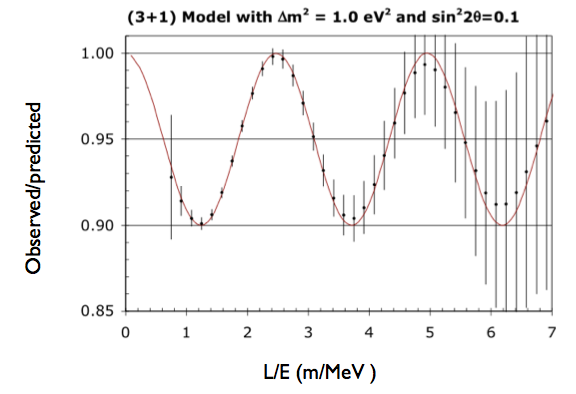
\includegraphics[width=0.80\textwidth]{./images/beyond3nu/future/isodar_wiggles.png}
  \end{column}
\end{columns}
\end{frame}

\begin{frame}[t]{Future accelerator-based projects: Isotope DAR neutrinos}
\centering
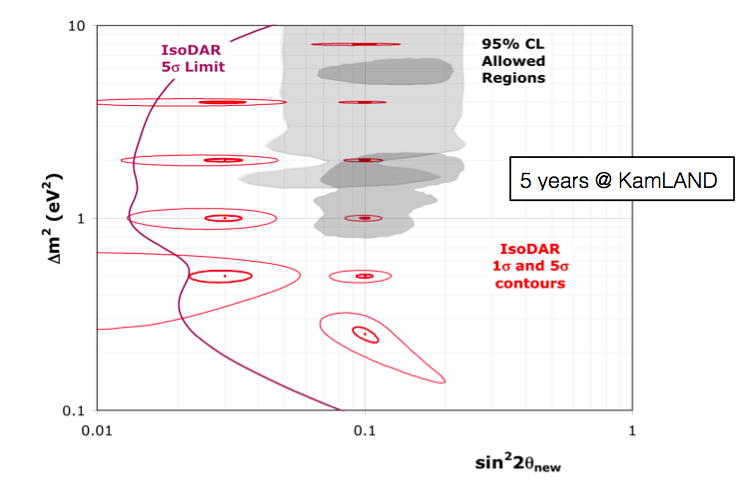
\includegraphics[width=0.96\textwidth]{./images/beyond3nu/future/isodar_sensitivity.png}
\end{frame}


\begin{frame}[t]{Future accelerator-based projects: $\mu$ DIF neutrinos}

\begin{columns}[t]
  \begin{column}{0.50\textwidth}
   {\scriptsize
     Entry-level neutrino factory {\color{blue}[FERMILAB-PROPOSAL-1028]}:
     \begin{itemize}
     {\scriptsize
       \item $\nu_{e}$ and $\nu_{\mu}$ beam from the decay of a stored muon beam
       \item Injecting 5 GeV pions into a muon storage ring
       \item Straight section of the ring is 185 m
       \item Pions that do not decay prior to first bent are removed
       \item Ring circulated muons with momenta of 3.8 GeV/c ($\pm$10\% momentum acceptance)
       \item 2$\times 10^{18}$ usefull muon decays (in the straight towards the detector)
             per $10^{21}$ protons on target.\\
     }
     \end{itemize}
     }
     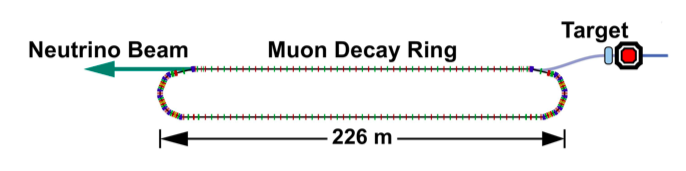
\includegraphics[width=0.99\textwidth]{./images/beyond3nu/future/nustorm.png}
  \end{column}
  \begin{column}{0.50\textwidth}
    \centering
     {\bf 10$\sigma$ sensitivity to the LSND+MiniBooNE anomaly} "with conservative systematics"\\
     \vspace{0.2cm}
     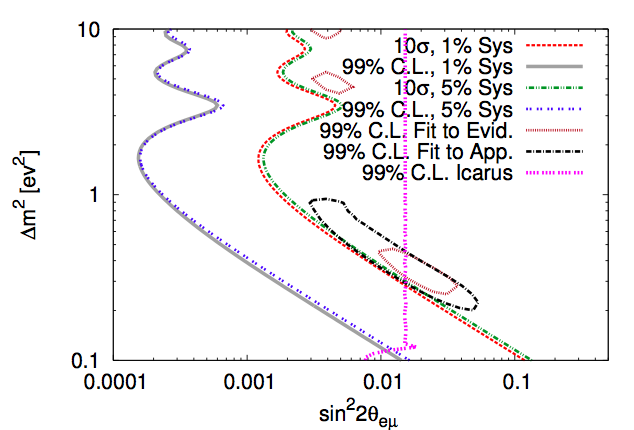
\includegraphics[width=0.95\textwidth]{./images/beyond3nu/future/nustorm_sensitivity.png}\\
     {\scriptsize \color{blue}[Phys.Rev. D89 (2014) 071301]}\\
  \end{column}
\end{columns}
\end{frame}


\begin{frame}[t]{Future accelerator-based projects: $\pi$,K DIF neutrinos}

\begin{center}
  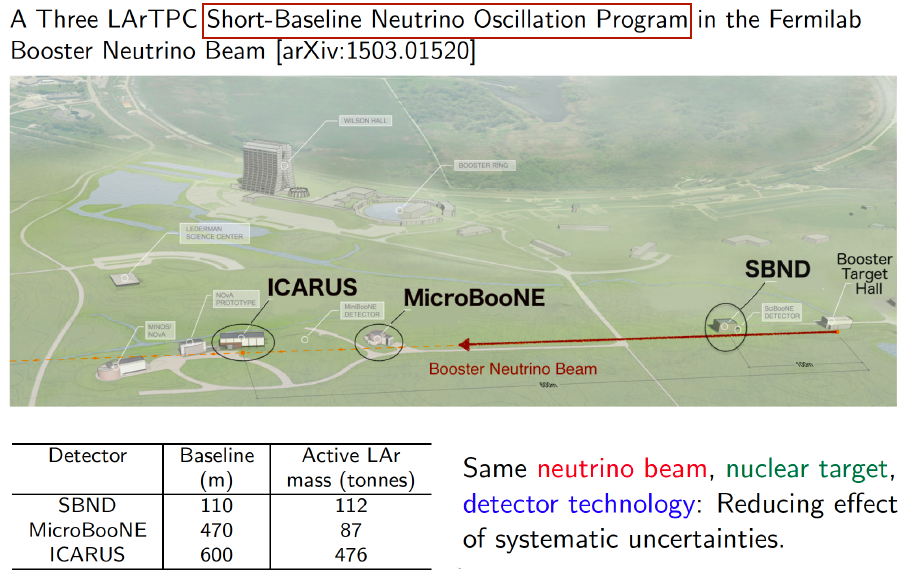
\includegraphics[width=0.95\textwidth]{./images/beyond3nu/sbn_1.png}\\
\end{center}
\end{frame}

\begin{frame}[t]{Future accelerator-based projects: $\pi$,K DIF neutrinos}

  {\small
    A definitive $>$5 $\sigma$ test of current anomalies is possible at SBN.\\
    Sensitivity is boosted by superb LArTPC imaging capabilities, and
    multiple identical detectors at different baselines.\\
  }

  \begin{columns}[T]
    \begin{column}{0.50\textwidth}
      \begin{center}
        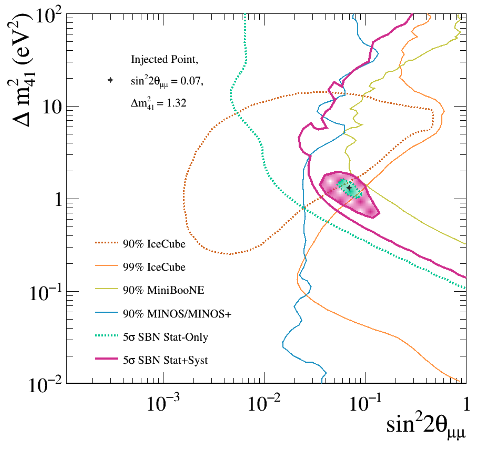
\includegraphics[width=0.99\textwidth]{./images/beyond3nu/sbn_a}
      \end{center}
    \end{column}
    \begin{column}{0.50\textwidth}
    \end{column}
  \end{columns}

\end{frame}

\begin{frame}[t]{Future accelerator-based projects: $\pi$,K DIF neutrinos}

  {\small
    A definitive $>$5 $\sigma$ test of current anomalies is possible at SBN.\\
    Sensitivity is boosted by superb LArTPC imaging capabilities, and
    multiple identical detectors at different baselines.\\
  }

  \begin{columns}[T]
    \begin{column}{0.50\textwidth}
      \begin{center}
        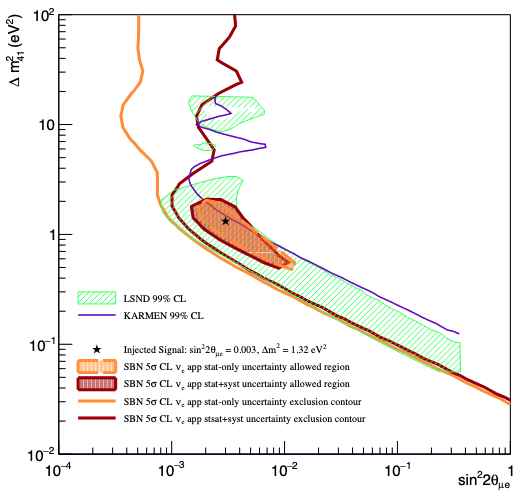
\includegraphics[width=0.99\textwidth]{./images/beyond3nu/sbn_b}
      \end{center}
    \end{column}
    \begin{column}{0.50\textwidth}
      \begin{center}
        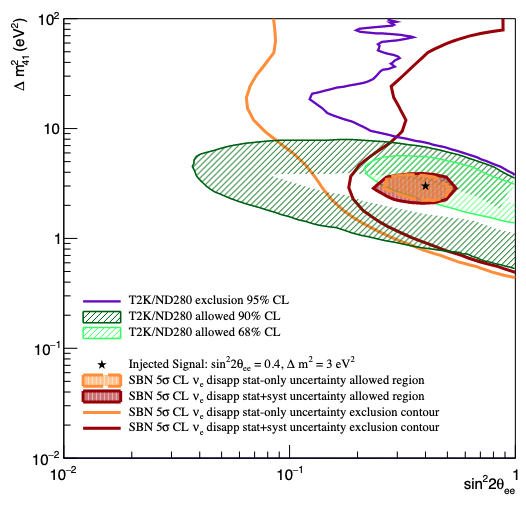
\includegraphics[width=0.99\textwidth]{./images/beyond3nu/sbn_c}
      \end{center}
    \end{column}
  \end{columns}

\end{frame}


%
%
%

% \begin{frame}{What to read}
%
% {\color{magenta} Add in next revision}
%
% \end{frame}
